\documentclass{beamer}

\usepackage[T1, T2A]{fontenc}
\usepackage[utf8]{inputenc}
\usepackage[english, russian]{babel}

\usetheme{Madrid}
\usecolortheme{beaver}
\setbeamertemplate{caption}[numbered]
\makeatother
\setbeamertemplate{footline}
{\leavevmode%
  \hbox{%
  \begin{beamercolorbox}[wd=.4\paperwidth,ht=2.25ex,dp=1ex,center]{author in head/foot}%
      \usebeamerfont{author in head/foot}\insertshortauthor{}~(\insertshortinstitute{})
  \end{beamercolorbox}%
  \begin{beamercolorbox}[wd=.5\paperwidth,ht=2.25ex,dp=1ex,center]{title in head/foot}%
    \usebeamerfont{title in head/foot}\insertshorttitle
  \end{beamercolorbox}%
  \begin{beamercolorbox}[wd=.1\paperwidth,ht=2.25ex,dp=1ex,center]{date in head/foot}%
    \insertframenumber{} / \inserttotalframenumber\hspace*{1ex}
  \end{beamercolorbox}}%
}
\makeatletter
\setbeamertemplate{navigation symbols}{}

\usepackage{animate}
\usepackage{graphicx}
\bibliographystyle{unsrt}

\usepackage{hyperref}
\hypersetup{colorlinks=true,
    linkcolor=blue,
    filecolor=magenta,
    urlcolor=cyan,
}

\usepackage{amssymb}
\usepackage{amsmath}
\usepackage{amsthm}
\usepackage{lscape}
\usepackage{color}
\graphicspath{{./images/}}

\AtBeginSection[]
{
    \begin{frame}
        \frametitle{Содержание}
        \tableofcontents[currentsection]
    \end{frame}
}

\title[3D реконструкция поверхности в СЭМ]{Трехмерная сканирующая электронная микроскопия
топографии поверхности с учетом влияния функции отклика детекторной системы:
математические методы обработки данных.}
\author[А.А.~Борзунов]{А.А.~Борзунов\inst{1} \and Д.В.~Лукьяненко\inst{1} \and Э.И.~Рау \inst{1} \and А.Г.~Ягола \inst{1}}
\institute[МГУ им. М.В. Ломоносова]{Московский Государственный Университет им. М.В. Ломоносова,
физический факультет}
\titlegraphic{
\includegraphics[width=2cm]{ff.png}}

\date{21 Апреля 2021 г.}



\begin{document}

\begin{frame}
    \titlepage
\end{frame}

%---------------------------------------------------------------------------------------------------

\section{Проблематика}
\begin{frame}
    \sectionpage
\end{frame}

\begin{frame}[c]
    \frametitle{Проблематика}
    \begin{columns}
        \begin{column}{0.5\textwidth}
            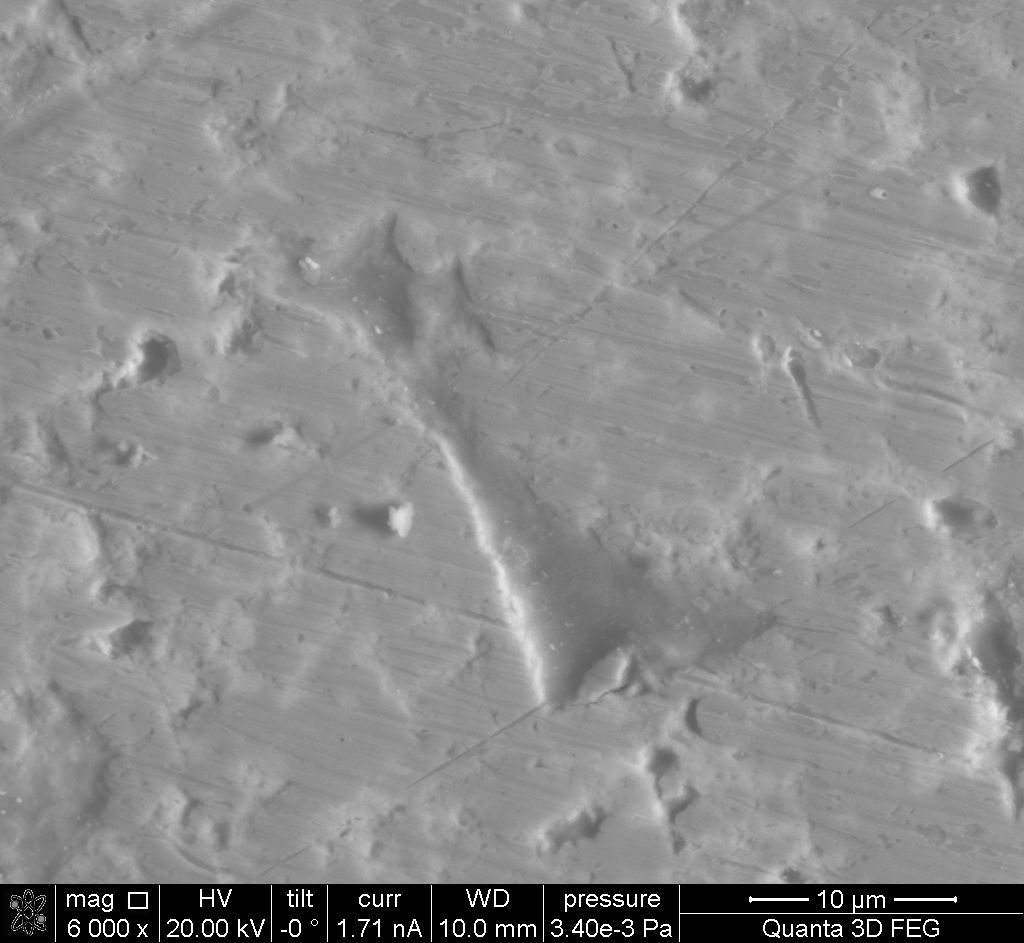
\includegraphics[width=1.0\linewidth]{VA.png}
        \end{column}
        \begin{column}{0.5\textwidth}
            % nothing here, will be in the next frame
        \end{column}
    \end{columns}
\end{frame}

% Создаем анимацию посредством копирования слайда :-)
\begin{frame}[c]
    \frametitle{Проблематика}
    \begin{columns}
        \begin{column}{0.38\textwidth}
            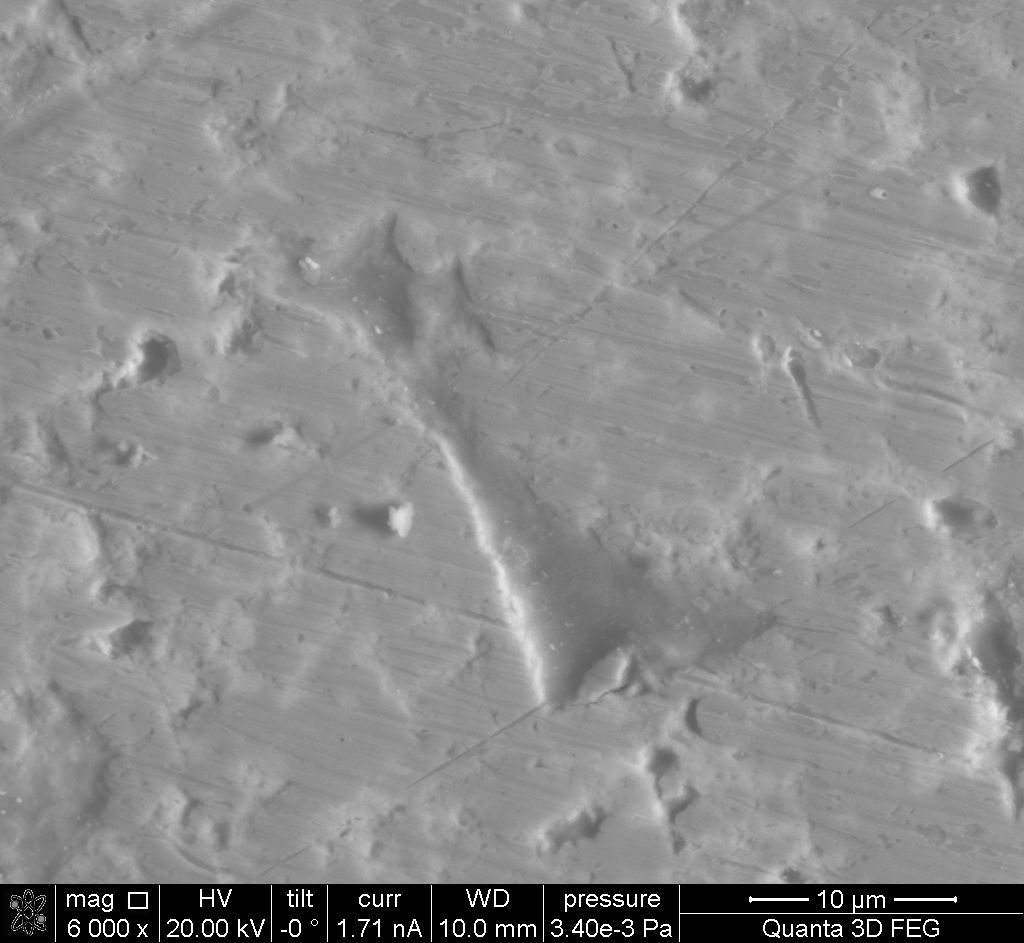
\includegraphics[width=1.0\linewidth]{VA.png}
        \end{column}
        \begin{column}{0.58\textwidth}
            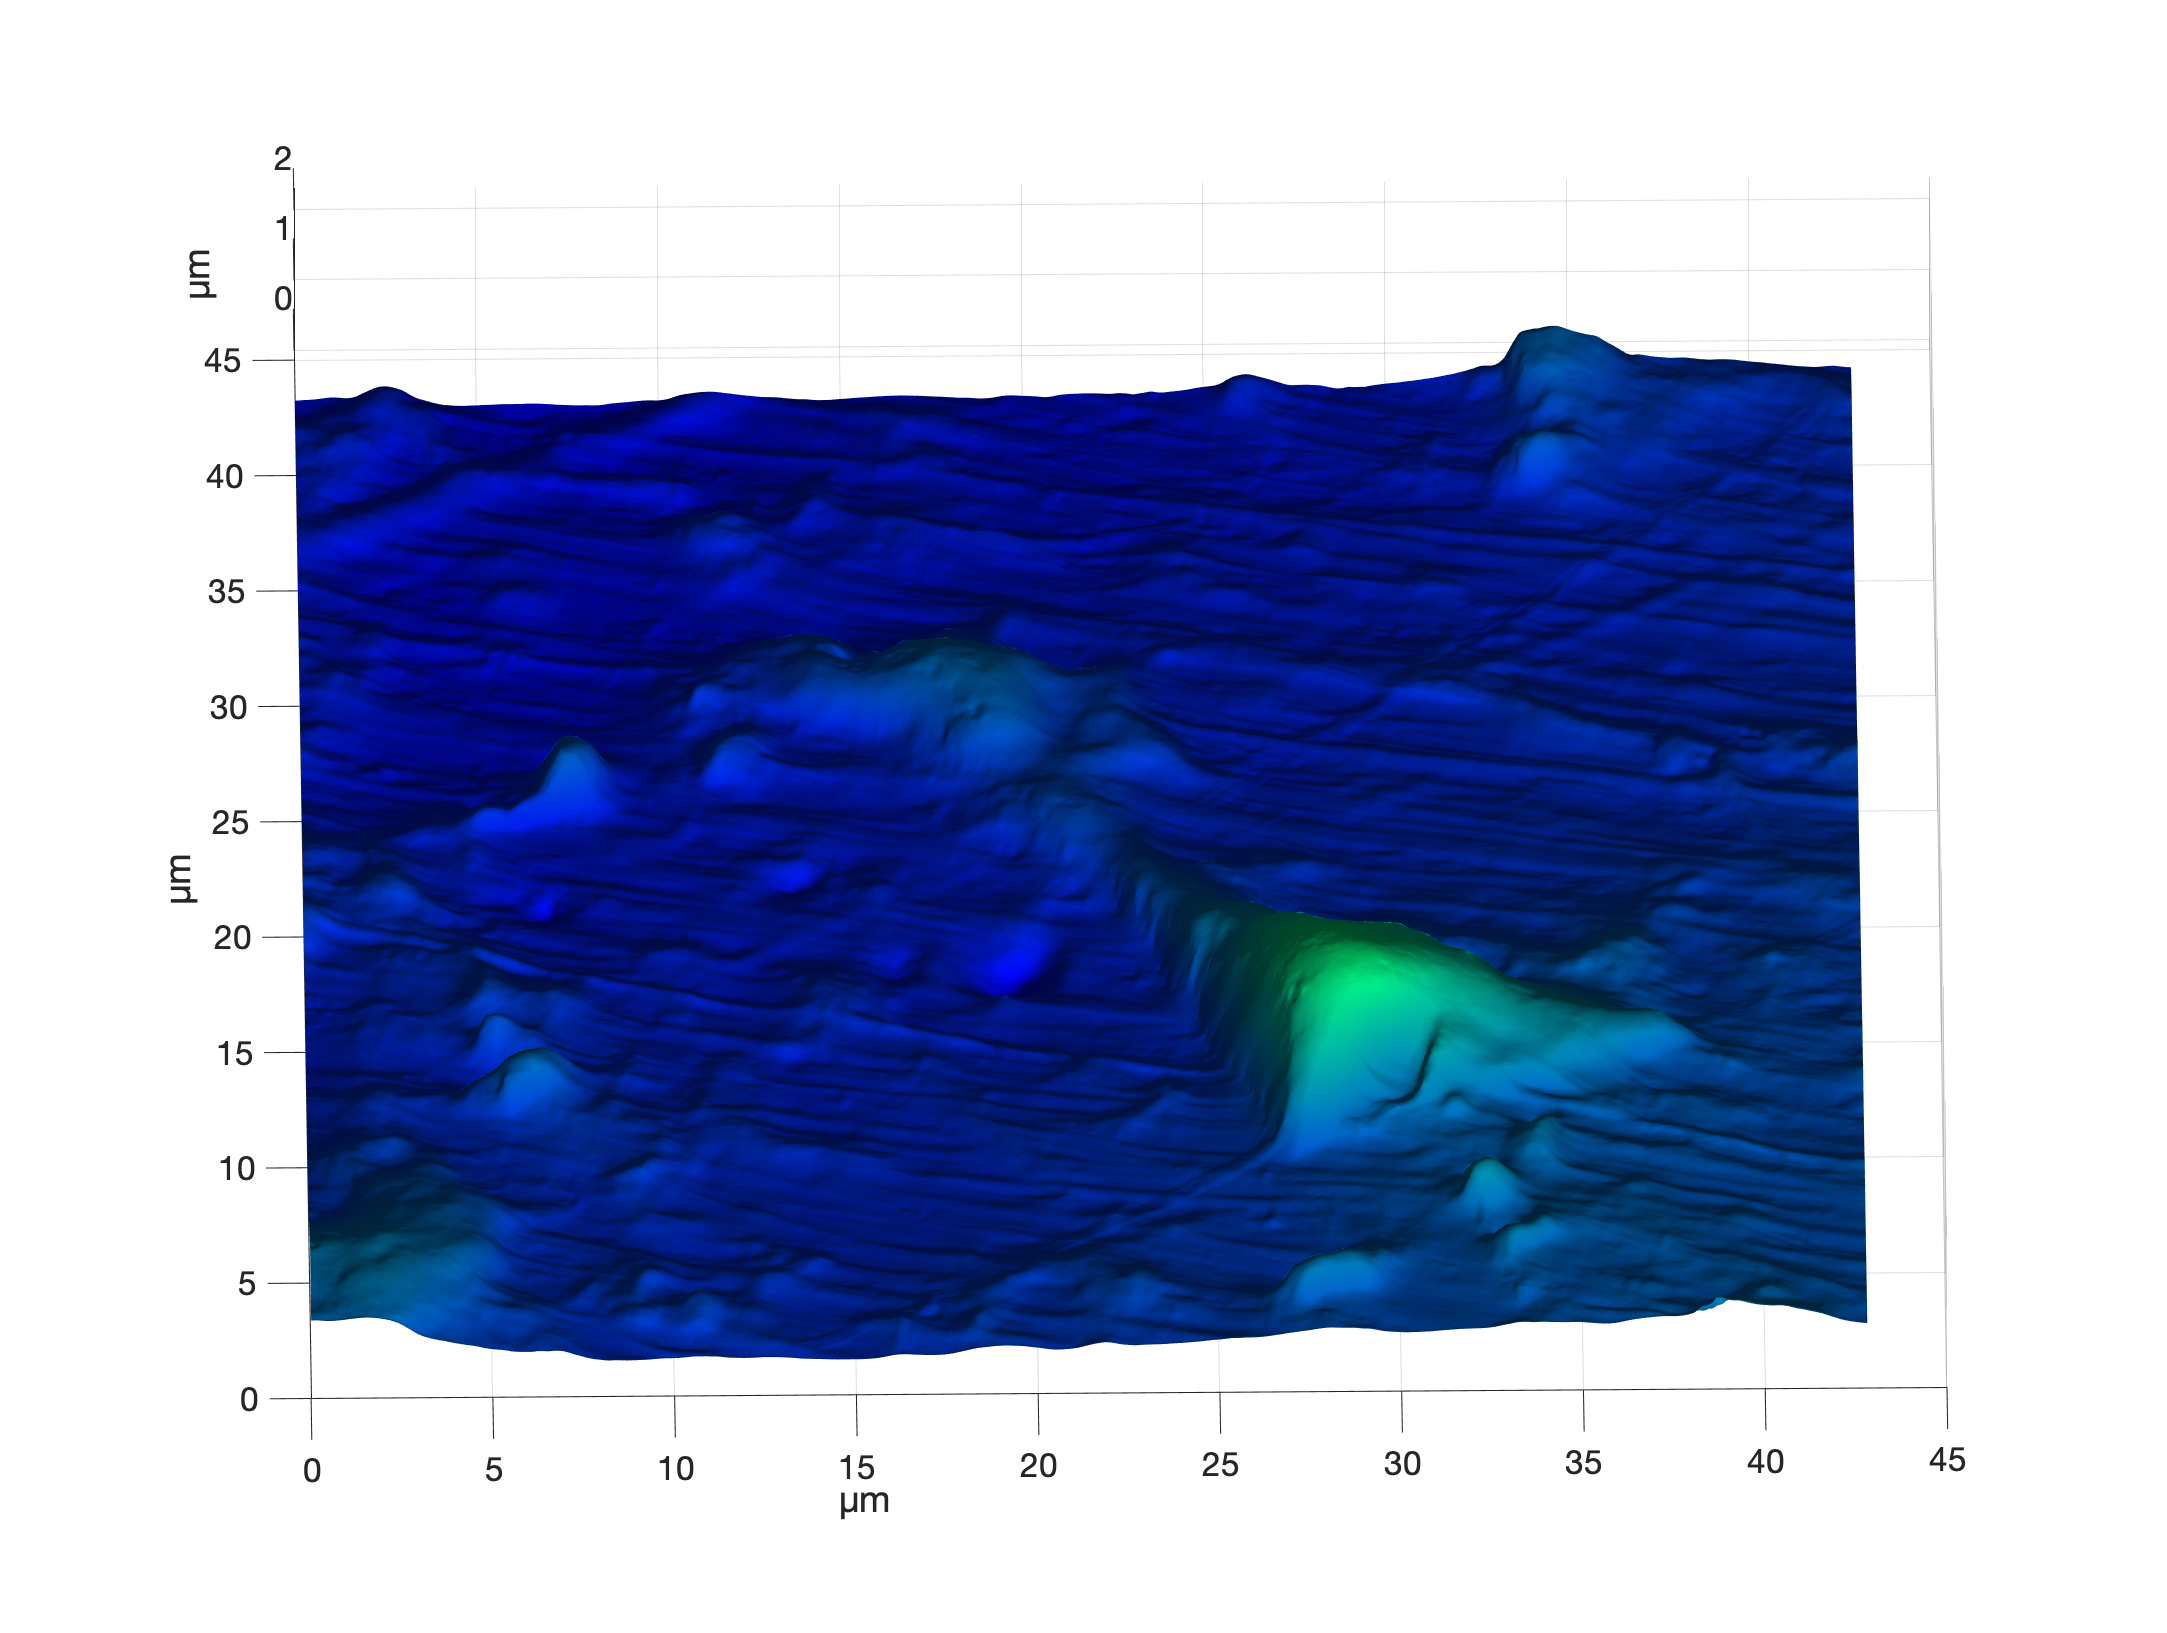
\includegraphics[width=1.0\linewidth]{tin-copper.eps}
        \end{column}
    \end{columns}
\end{frame}

\begin{frame}
    \frametitle{Экспериментальная установка}
    \begin{figure}
        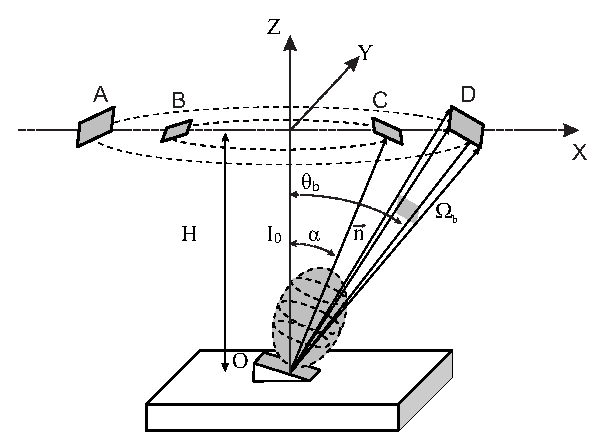
\includegraphics[width=0.6\linewidth]{detector_structure.eps}
        \caption{Устройство детектора в плоскости $X$: $\alpha$~--- угол между нормалью малого
участка поверхности и электронным лучом $I_0$, $A,B,C,D$~--- детекторы, O-образец,
$\Omega_{d}$~--- телесный угол детектора $D$ отклоненного на угол $\theta_d$, $H$~--- рабочее
расстояние СЭМ.}
        {\label{fig:detector_structure}}% chktex 8
    \end{figure}
\end{frame}

\begin{frame}
    \frametitle{Постановка задачи}
    Согласно~\cite{PaluszynskiSlowko2005Vacuum, DrzazgaPaluszynski2005Measurement} интенсивность
    разностного сигнала связана с углом наклона соответствующего участка поверхности:
    \begin{equation*}
        I_{AB} = \frac{I_A - I_B}{I_A + I_B} \sim \tan{\alpha^x}, \quad
        I_{EF} = \frac{I_E - I_F}{I_E + I_F} \sim \tan{\alpha^y}
    \end{equation*}
    \textbf{Задача 1:} Сигнал $I_{AB}(x,y), I_{EF}(x,y)$ в области $P$ предполагается известным.
    Необходимо восстановить градиент поверхности
    $
        \left(\frac{\partial Z}{\partial x}(x,y), \frac{\partial Z}{\partial y} (x,y) \right),
        (x,y) \in S
    $.

    \vfill

    \textbf{Задача 2:} Градиент
    \begin{equation}
        {\Big(\frac{\partial Z}{\partial x}(x,y),
        \frac{\partial Z}{\partial y} (x,y)\Big)}^{T} =
        {\big(J_x(x,y), J_y(x,y)\big)}^T, \quad (x,y) \in S
        \label{eq:problem_statement}
    \end{equation}
    предполагается известным. Найти функцию $Z(x,y)$ представляющую восстанавливаемую поверхность.
\end{frame}

%---------------------------------------------------------------------------------------------------

%---------------------------------------------------------------------------------------------------
\section{Восстановление градиента}
\begin{frame}
    \sectionpage
\end{frame}


\begin{frame}[c,allowframebreaks]
    \frametitle{Восстановление градиента}

    Применяя метод калибровочной поверхности (рис.~\ref{fig:inputSphere}), описанный в~\cite{main},
необходимо восстановить аппаратные функции $F_x, F_y$ (рис~\ref{fig:Tables})).

    \begin{figure}[hp]
        \includegraphics[width=0.7\linewidth]{S.eps}
        \caption{\small Разностный сигнал $I_{AB}$ в направлении сканирования вдоль
        оси $x$~(a) и $y$~(b).}
        {\label{fig:inputSphere}}% chktex 8
    \end{figure}

    \framebreak

    Исследуемая область представляется в виде матриц $K^x$, $K^y$ размером $(N,N)$,
элементами которых является интенсивность сигнала $k^x (i,j)$, $k^y (i,j)$ в точке $(x_j, y_i)$.

    Для каждого элемента $k^x_{i,j}$ матрицы $K^x$, который принадлежит калибровочной поверхности,
найдем производную $\frac{\partial z}{\partial x} \big|_{(x_j,y_i)} $ аналитически, таким
образом составляя таблицу, задающую сеточные значения функции обратной к аппаратной функции
$\hat{F^x}$ зависимости сигнала $K^x_{i,j} = F^x (\tan(\alpha^x_{i,j}))$ от угла наклона
поверхности $\alpha^x$ к оси $x$.
    \begin{center}
        \begin{tabular}{| c| c |}
            \hline
            $ k^x_{i,j} $ & $ \tan{ \frac{\partial z(x_j, y_i)}{\partial x} } $ \\
            \hline
            \vdots          & \vdots \\
            \hline
            $ k^x_{i',j'} $ & $ \tan{ \frac{\partial z(x_{j'}, y_{i'})}{\partial x} } $ \\
            \hline
        \end{tabular}
    \end{center}

    \framebreak

    \begin{figure}
        \includegraphics[width=0.9\linewidth]{Tables.eps}
        \caption
        {
            График аппаратных функций $F^x$, $F^y$ зависимости угла наклона поверхности
            (в градусах) от интенсивности сигнала. И их табличного представления
            $\hat{F^x}$, $\hat{F^y}$
        }
        {\label{fig:Tables}}% chktex 8
    \end{figure}

    \framebreak

    \begin{figure}
        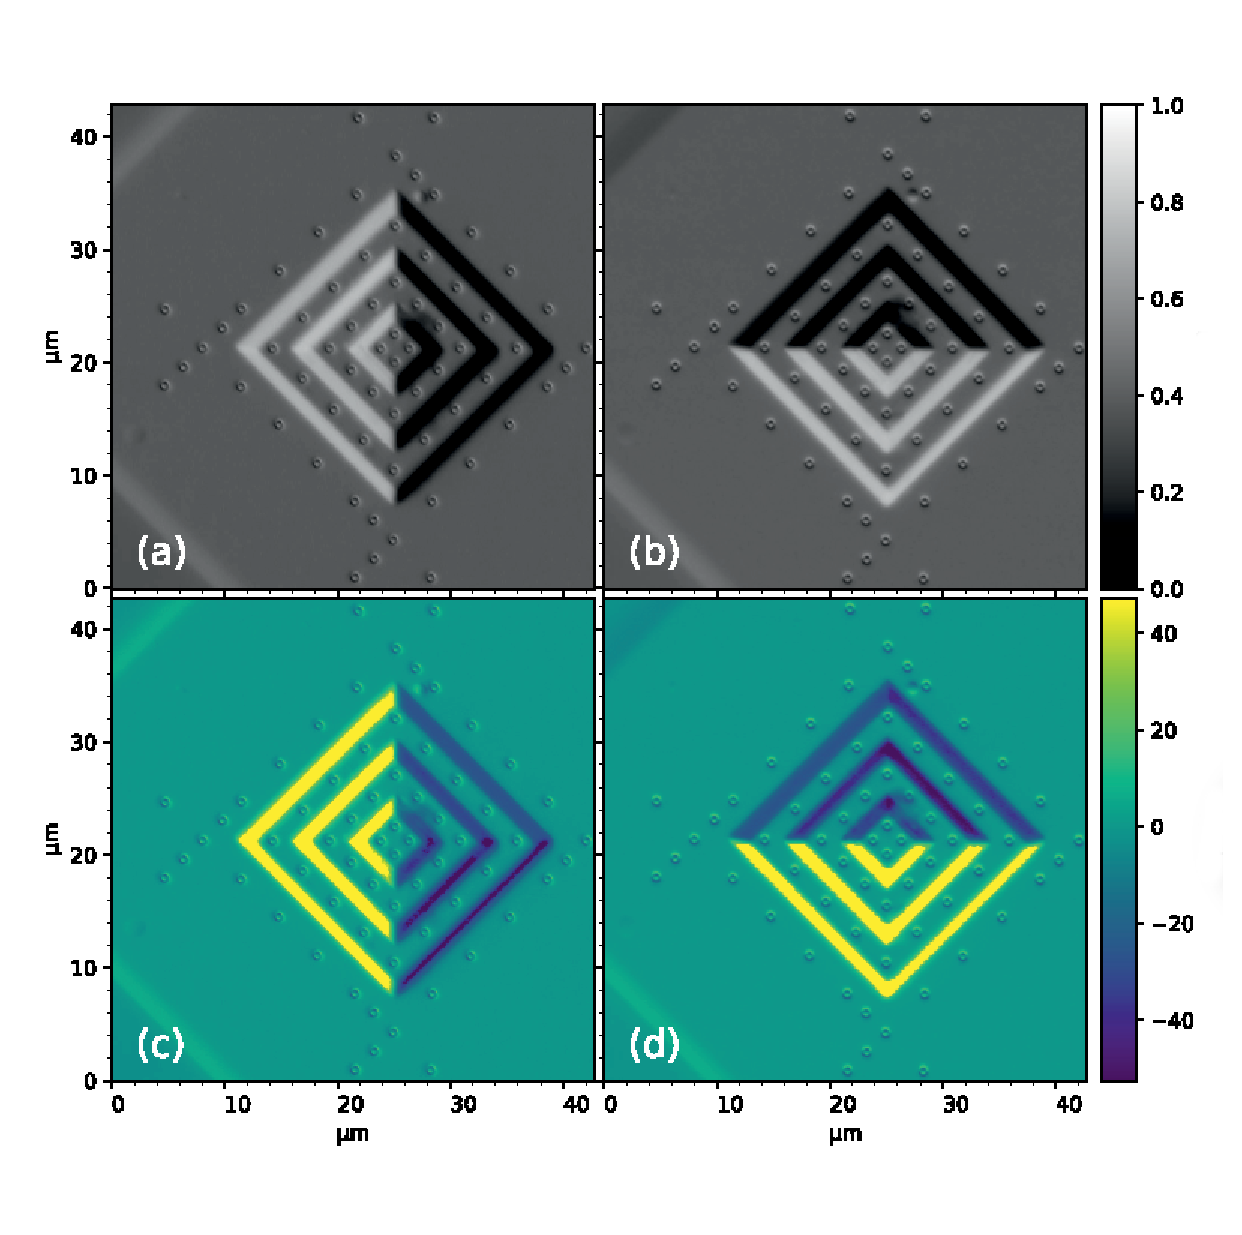
\includegraphics[width=0.5\linewidth]{P.eps}
        \caption{Входные изображения (a) и (b) восстанавливаемой поверхности и её карта углов (c) и (d).}
        {\label{fig:input_data}}% chktex 8
    \end{figure}
\end{frame}
% --------------------------------------------------------------------------------------------------


% --------------------------------------------------------------------------------------------------
% --------------------------------------------------------------------------------------------------
% --------------------------------------------------------------------------------------------------
\section{Восстановление поверхности}
\begin{frame}
    \sectionpage
\end{frame}


\begin{frame}[c,allowframebreaks]
    \frametitle{Восстановление поверхности}

    Исходная задача~(\ref{eq:problem_statement}) может быть сформулирована в операторном виде
    следующим образом~\cite{second}
    \begin{equation*}
        \label{operator_equation_0}
        A[Z] = {\textbf{\emph{J}}},
    \end{equation*}
где оператор $A: W_2^2(S) \to L_2(S)$ непрерывен. Этот оператор отображает искомую функцию $Z(x,y)$
представляющую исследуемую трехмерную поверхность образца в её градиент ${\textbf{\emph{J}}}$.
В ходе измерений градиента ${\textbf{\emph{J}}}$ мы получаем его приближенное значение
$\textbf{\emph{J}}_\delta$, такое что верна ошибка измерений $\delta$ удовлетворяет оценке
$\|{\textbf{\emph{J}}}_\delta - {{\textbf{\emph{J}}}}\|_{L_2}\leq\delta$.

    \framebreak

    Таким образом, образом обратная задача восстановления трехмерной поверхности может быть
    сформулирована в следующем виде:
    \begin{equation}
        \label{eq:operator_equation}
        A[Z_\delta] = {\textbf{\emph{J}}}_\delta, \quad {\textbf{\emph{J}}}_\delta \in L_2(S).
    \end{equation}

    Решение задачи~(\ref{eq:operator_equation}) следует искать в виде элемента $Z_\delta \in W_2^2(S)$,
    реализующего минимум функционала
    \begin{equation}
        \label{functional}
        F[Z] = \big\|A[Z] - {\textbf{\emph{J}}}_\delta\big\|_{L_2}^2.
    \end{equation}
\end{frame}
% --------------------------------------------------------------------------------------------------
% --------------------------------------------------------------------------------------------------
% --------------------------------------------------------------------------------------------------




% --------------------------------------------------------------------------------------------------
% --------------------------- N U M E R I C A L   R E A L I Z A T I O N ----------------------------
% --------------------------------------------------------------------------------------------------
\section{Численная реализация}
\begin{frame}
    \sectionpage
\end{frame}

\begin{frame}[c,allowframebreaks]
    \frametitle{Численная реализация}

    Входные данные ((a) and (b) at рис.~\ref{fig:input_data}) представляются в виде матриц
    $K^x$, $K^y$ размера $(N \times N)$, элементами которых являются интенсивности разностных
    сигналов $k^x_{i,j} \equiv K^x (i,j)$, $K^y_{i,j} \equiv k^y (i,j)$
    в точках $(x_j, y_i) \in S$, $i,j = \overline{1,N}$, значения которых нормированы на единицу.
    Поэлементно применяя к элементам матриц соответствующие обратные аппаратные функции получим
    значения компонент $J_x$ and $J_y$ градиента ${\textbf{\emph{J}}}$: $j^x_{i,j}$,
    $k^y_{i,j}$ в каждой точке $(x_j, y_i) \in S$, $i,j = \overline{1,N}$ исследуемой области.

    Для восстановления топографии поверхности необходимо переписать
    задачу~(\ref{eq:operator_equation}) в виде конечномерного аналога, дополнив её начальным
    условием $Z(x_0,y_0) = 0$, для произвольной точки $(x_0, y_0)$.

    \framebreak

    Таким, образом необходимо решить следующую задачу
    \begin{equation}
        \label{system_of_equations}
        \left\{
            \begin{aligned}
                &\nabla Z(x,y) = (J_x, J_y)^T, \quad (x,y)\in S, \\
                &Z(x_0,y_0) = 0.
            \end{aligned}
        \right.
    \end{equation}

    \framebreak

    Для этого необходимо переупорядочить матрицу $X$ компоненты градиента по столбцам
    \begin{equation}
        \label{column-major_ordering}
        J_x \equiv
        \left(
            \begin{array}{cccc}
                j^x_{1,1} & j^x_{1,2} & \cdots & j^x_{1,N} \\
                j^x_{2,1} & j^x_{2,2} & \cdots & j^x_{2,N} \\
                \vdots & \vdots & \ddots & \vdots  \\
                j^x_{N,1} & j^x_{N,2} & \cdots & j^x_{N,N}
            \end{array}
        \right)
        \sim
        \left(
            \begin{array}{c}
                j^x_{1,1} \\
                j^x_{2,1} \\
                \vdots \\
                j^x_{N,1} \\
                j^x_{1,2} \\
                j^x_{2,2} \\
                \vdots \\
                j^x_{N,2} \\
                \vdots \\
                j^x_{1,N} \\
                \vdots \\
                j^x_{N,N}
            \end{array}
        \right)
        \equiv{}  B^x.
    \end{equation}
    Выполняя аналогичное действие со второй компонентой градиента $J_y$ получим $B_y$, с искомой
    функцией $Z$~--- $\hat{Z}$.


    Что позволит нам записать задачу в матричном виде следующим образом:
    \begin{equation*}
        \label{matrix_equation}
        \hat{A} \hat{Z}  =
        \left(
        \begin{aligned}
            &B^x\\
            &B^y
        \end{aligned}
        \right)
        \equiv B.
    \end{equation*}
    Здесь матрица $\hat{A}$ размера $(2N^2 \times N^2)$ представляет конечно разностную апроксимацию
    частной производной $\frac{\partial}{\partial x}$ (первые $N^2$ строк) и
    $\frac{\partial}{\partial y}$ (последние $N^2$ строк).

    \framebreak

    \small
    \begin{equation*}
        \begin{array}{lllll}
            a_{i,i}             & = &-1/h & for & i = \overline{1,N^2},                         \\
            a_{i,i+N}           & = &1/h  & for & i = \overline{1,N^2 - N},                     \\
            a_{i,i-N}           & = &1/h  & for & i = \overline{N^2 - N,N^2 },                  \\
            a_{N^2+i+j, i+j}    & = &-1/h & for & i = 1, N+1, 2N+1,~\dots, (N-1)N + 1,          \\
                                &   &       &   & j = \overline{0,N-2},                         \\
            a_{N^2+i+j, i+j+1}  & = &-1/h & for & i = 1, N+1, 2N+1,~\dots, (N-1)N + 1,          \\
                                &   &       &   & j = \overline{0,N-2},                         \\
            a_{N^2+i+N-1, i+N-1} &= &-1/h & for & i = 1, N+1, 2N+1,~\dots, (N-1)N + 1,          \\
            a_{N^2+i+N-1, i+N-2} &= &1/h  & for & i = 1, N+1, 2N+1,~\dots, (N-1)N + 1,
        \end{array}
    \end{equation*}
    где $h$ постоянное расстояние между смежными точками сканирования в исходном изображении.
    Оно считается постоянным и одинаковым вдоль оси $X$ и $Y$.
    \normalsize

    \framebreak

    С помощью метода наименьших квадратов следует найти переупорядоченный по столбцам вектор
    сеточного представления искомой функции, представляющей поверхность исследуемого образца.
    \begin{equation*}
        \hat{Z} = \operatorname{argmin}\limits_Z \|\hat{A} Z - B\|^2.
    \end{equation*}

\end{frame}
% --------------------------------------------------------------------------------------------------

% --------------------------------------------------------------------------------------------------
% -------------------------------- G A L L E R Y ---------------------------------------------------
% --------------------------------------------------------------------------------------------------
\section{Примеры восстановления поверхностей}
\begin{frame}
    \sectionpage
\end{frame}

\begin{frame}[c,allowframebreaks]
    \frametitle{Результаты восстановления}

    \begin{figure}[ht]
        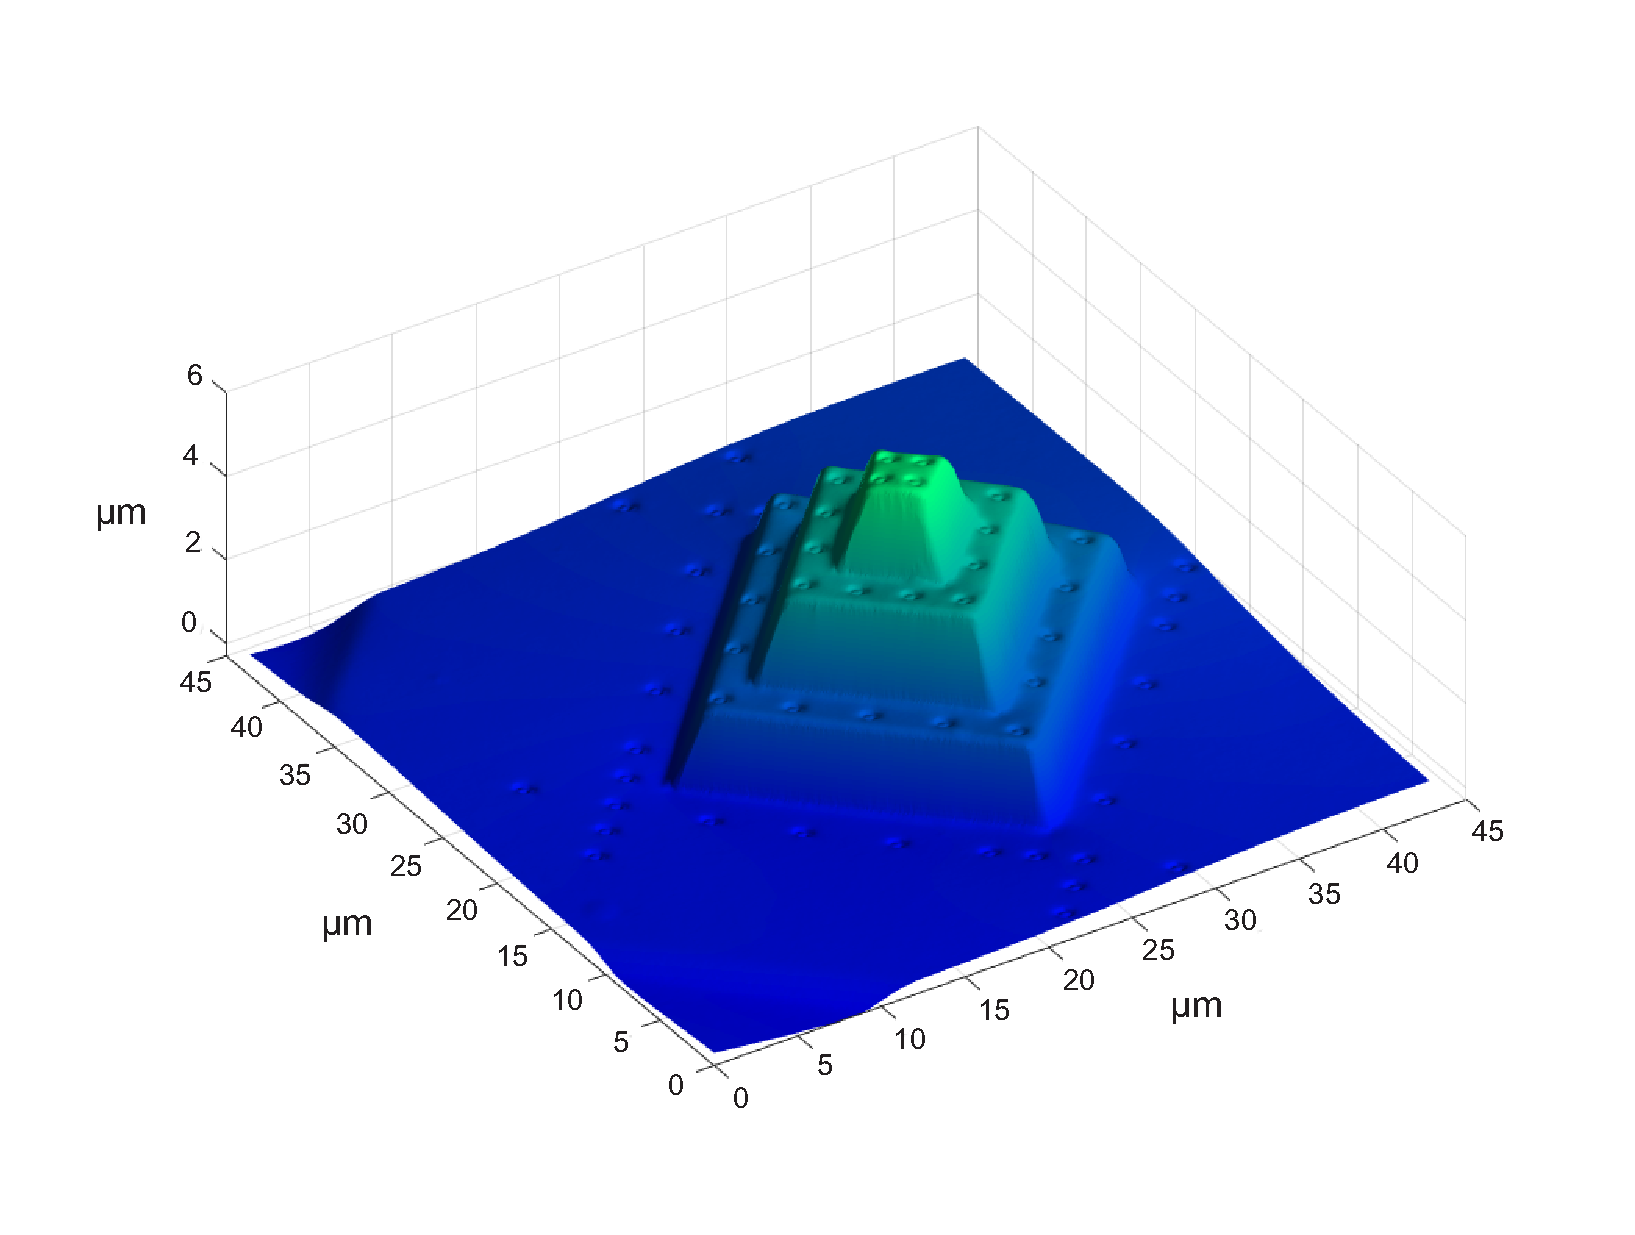
\includegraphics[width=0.65\linewidth]{berger.eps}
        \caption{Восстановленное изображение поверхности образца для тестирования СЭМ, входные
        изображения которого изображены на рис.~\ref{fig:input_data}.}
        {\label{fig:berger}}% chktex 8
    \end{figure}

\framebreak

    \begin{figure}[ht]
        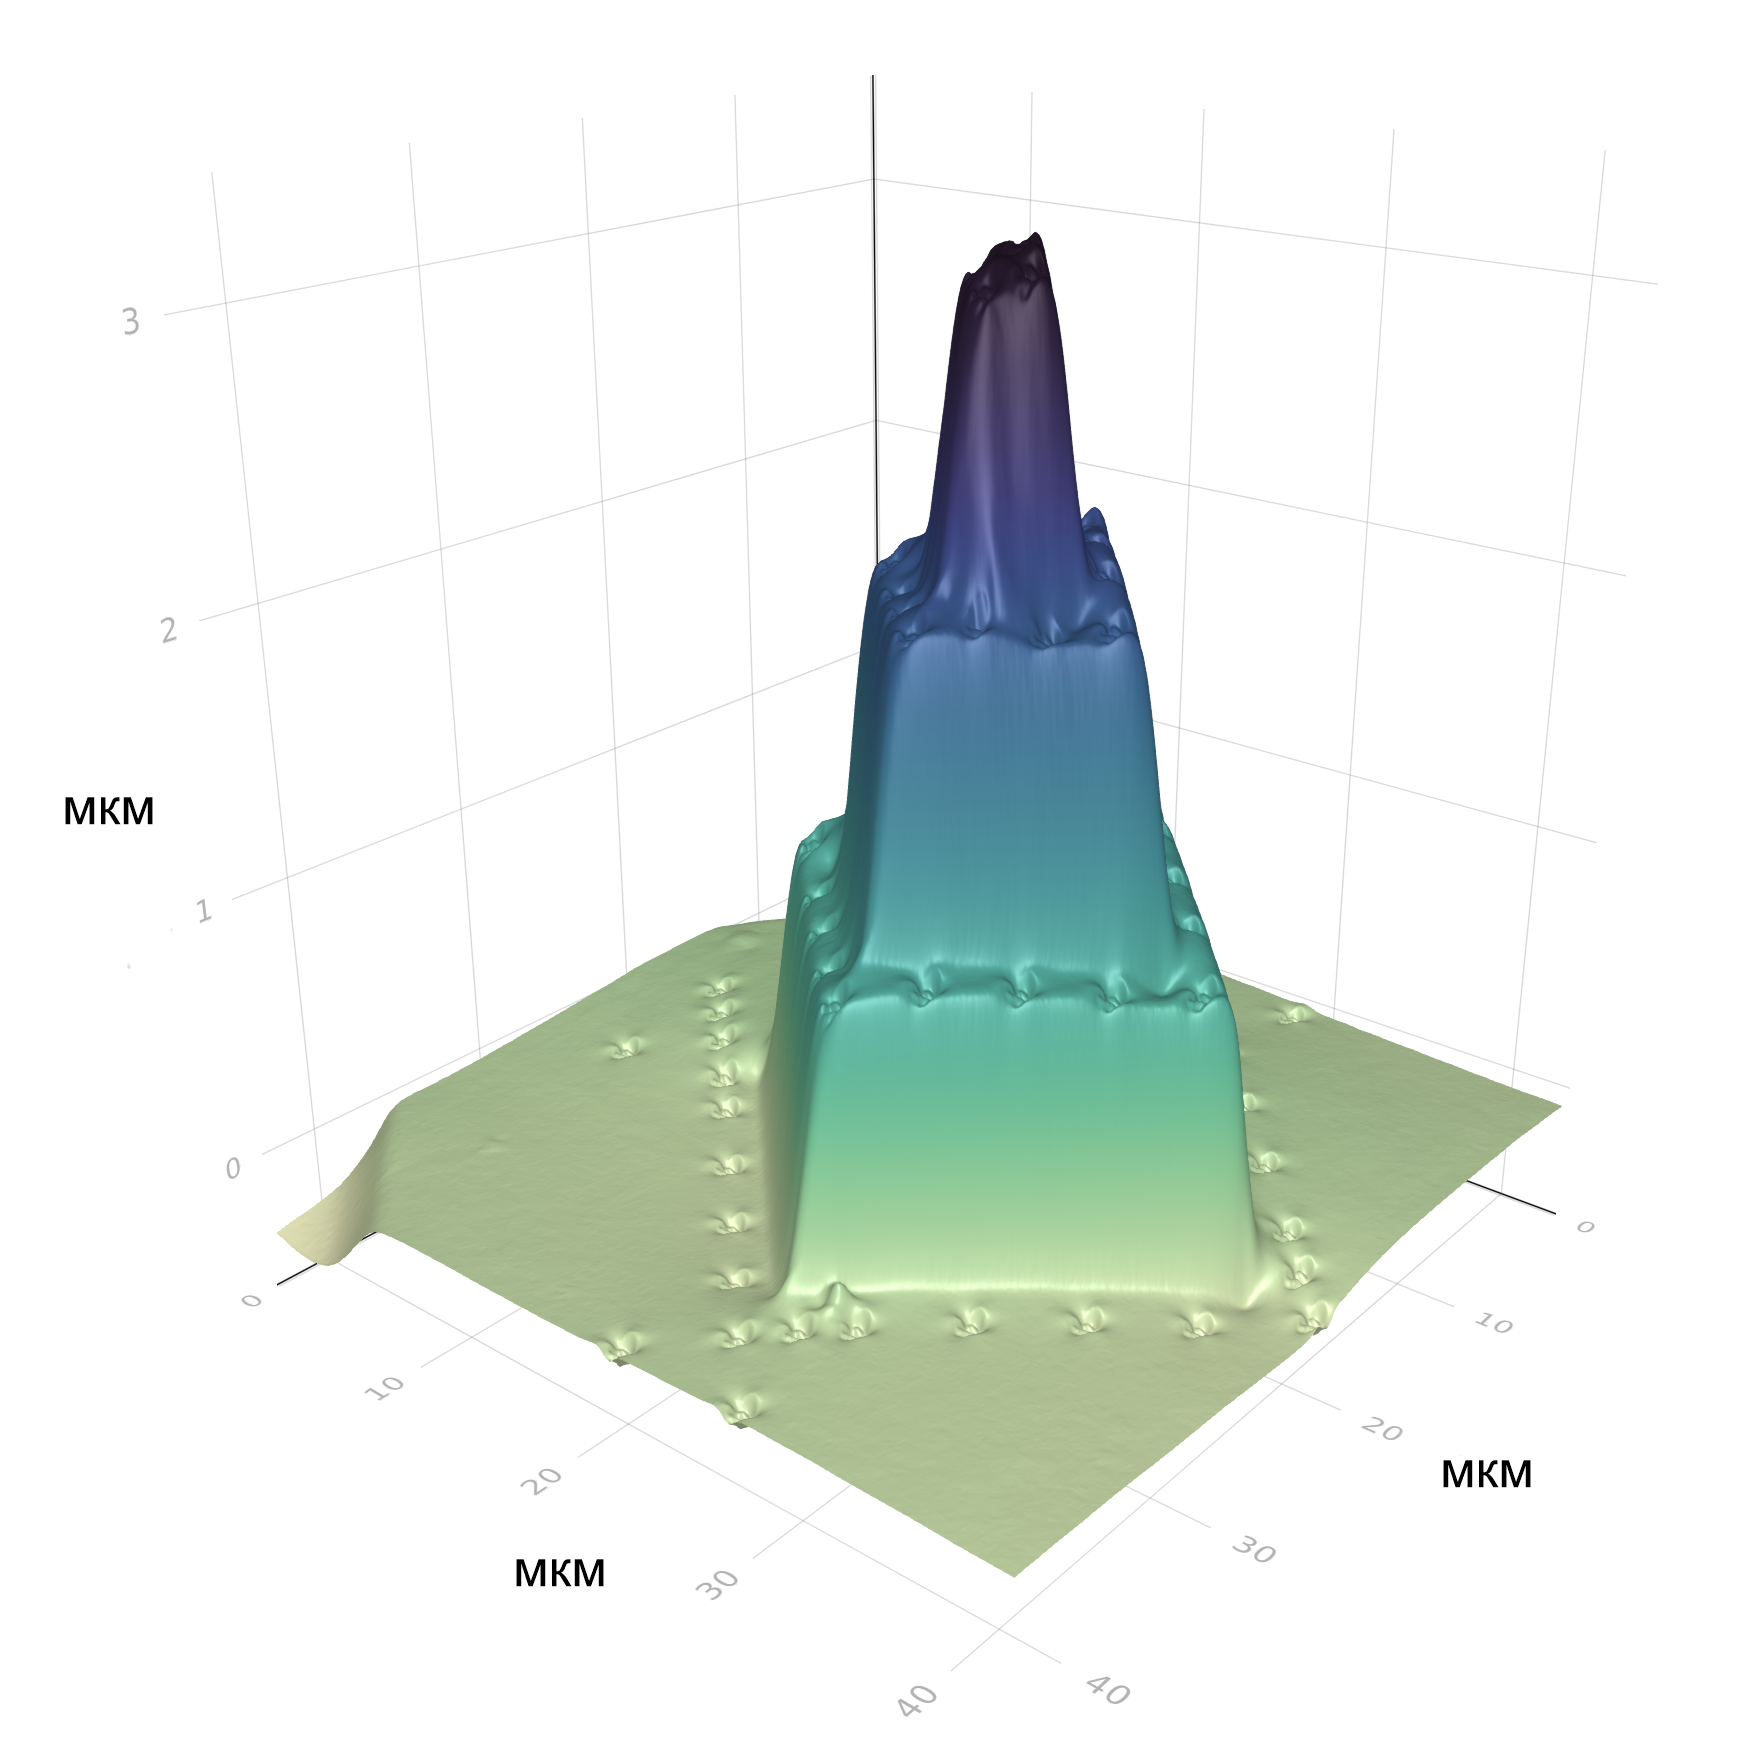
\includegraphics[width=0.55\linewidth]{pyramid_rotated.png}
    \end{figure}

\framebreak

    \begin{figure}[ht]
        \includegraphics[width=0.7\linewidth]{input_data2.eps}
        \caption{Разностный сигнал полученный с помощью СЭМ в режиме детектирования отраженных
            электронов вдоль оси $X$ (a), оси $Y$ (b). На снимках изображена серебреная пластина
            после теста твердости по Виккерсу. Профилограмма сигнала вдоль выделенной синем линии
            изображена на рис.~\ref{fig:results}.}
        {\label{fig:input_data2}}%
    \end{figure}

\framebreak

    \begin{figure}[t]
        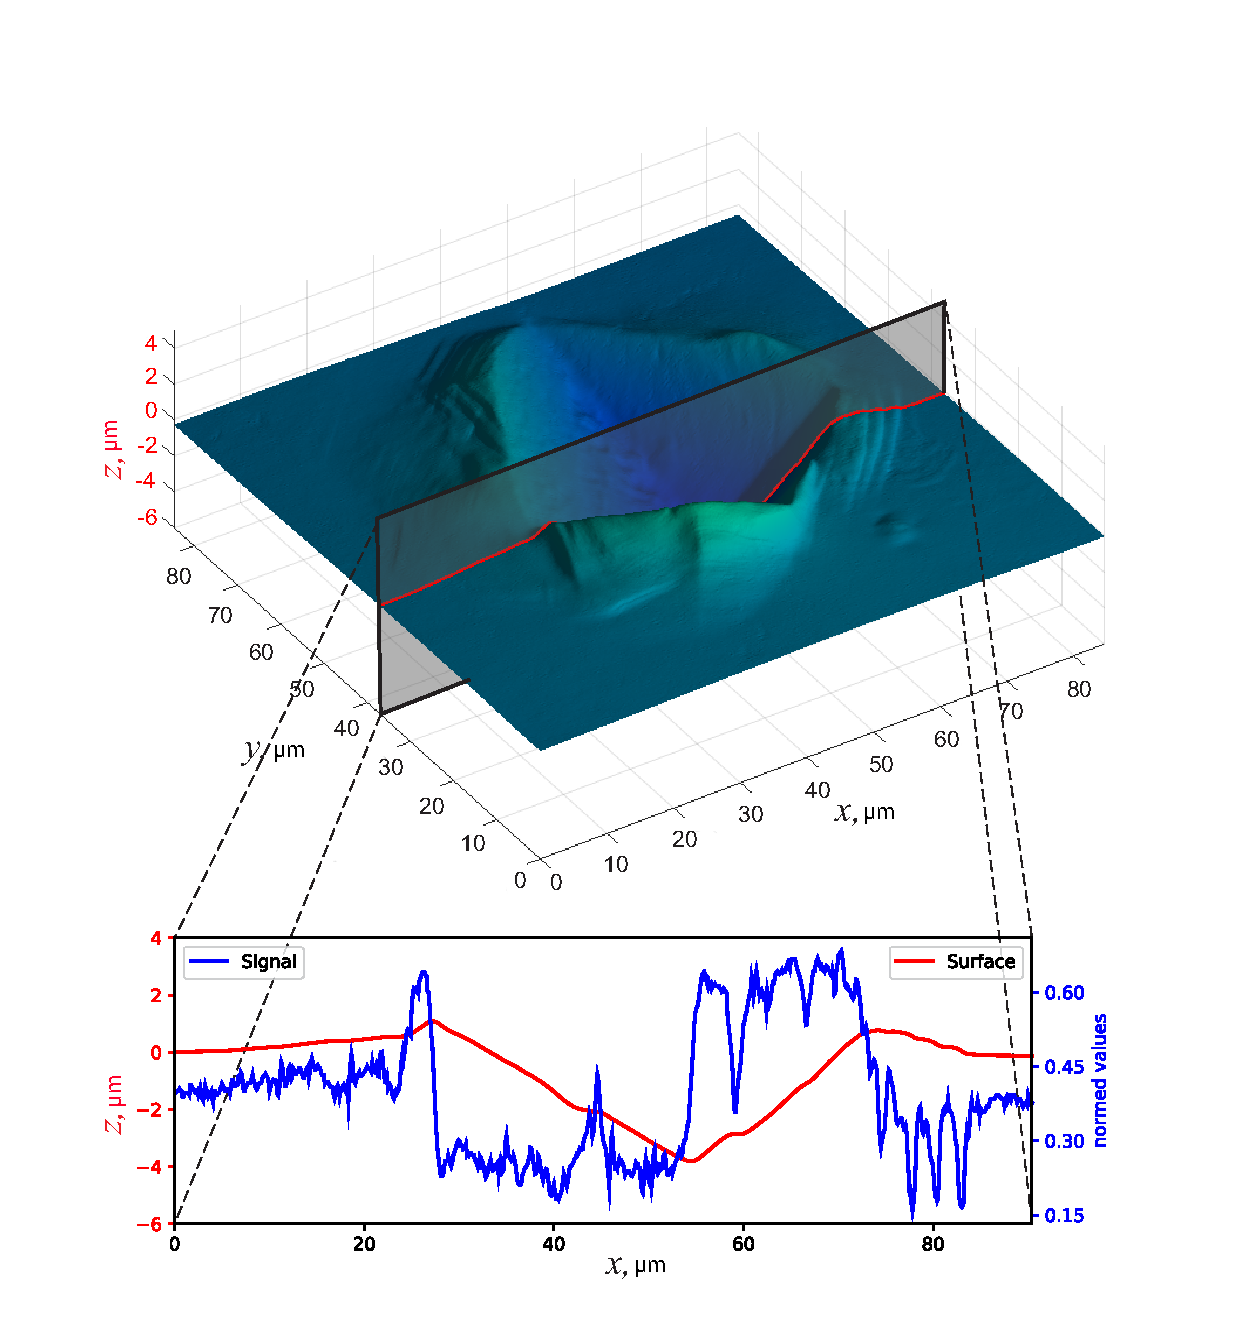
\includegraphics[width=0.40\linewidth]{results.eps}
        \caption{Восстановленная поверхность, входной сигнал на которой изображен на
            рис.~\ref{fig:input_data2}.}
        {\label{fig:results}}
    \end{figure}

\framebreak

    \begin{figure}[ht]
        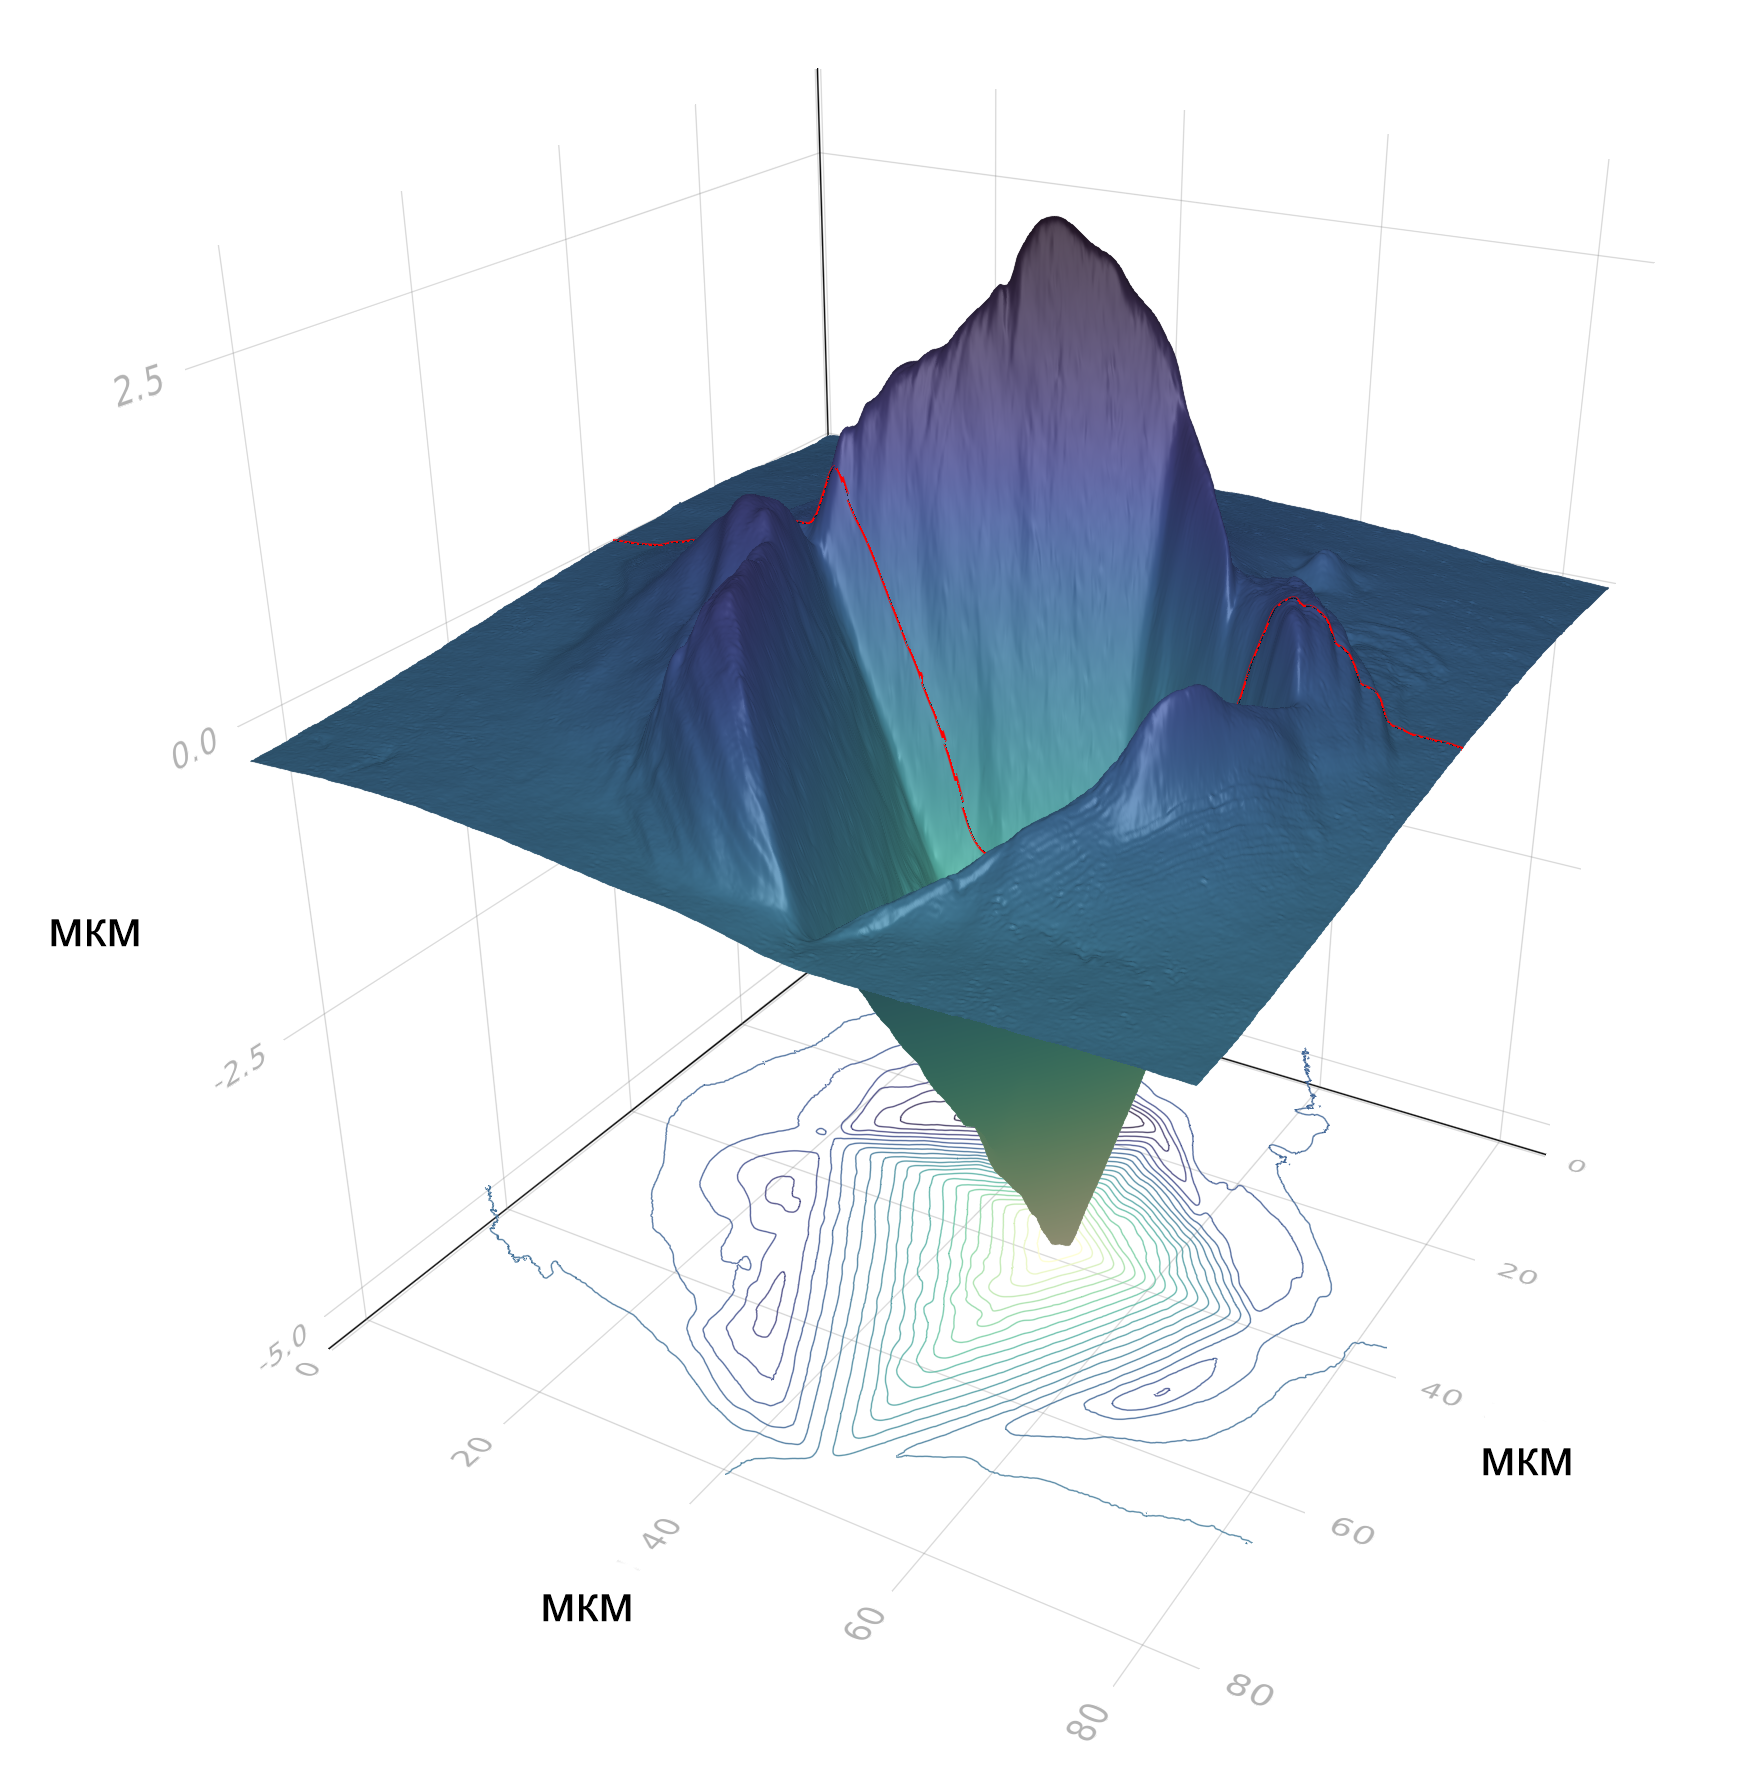
\includegraphics[width=0.55\linewidth]{crooked.png}
    \end{figure}

\framebreak

    \begin{figure}
        \includegraphics[width=0.8\linewidth]{indentor-source.eps}
        \caption{Разностный сигнал полученный с помощью СЭМ в режиме детектирования отраженных
            электронов вдоль оси $X$ (a), оси $Y$ (b). На снимках изображена серебреная пластина
            после теста твердости по Виккерсу. Профилограмма сигнала вдоль выделенной синем линии
        изображена на рис.~\ref{fig:indentor}.}% chktex 8
        \label{fig:indentor-source}
    \end{figure}

\framebreak

    \begin{figure}
        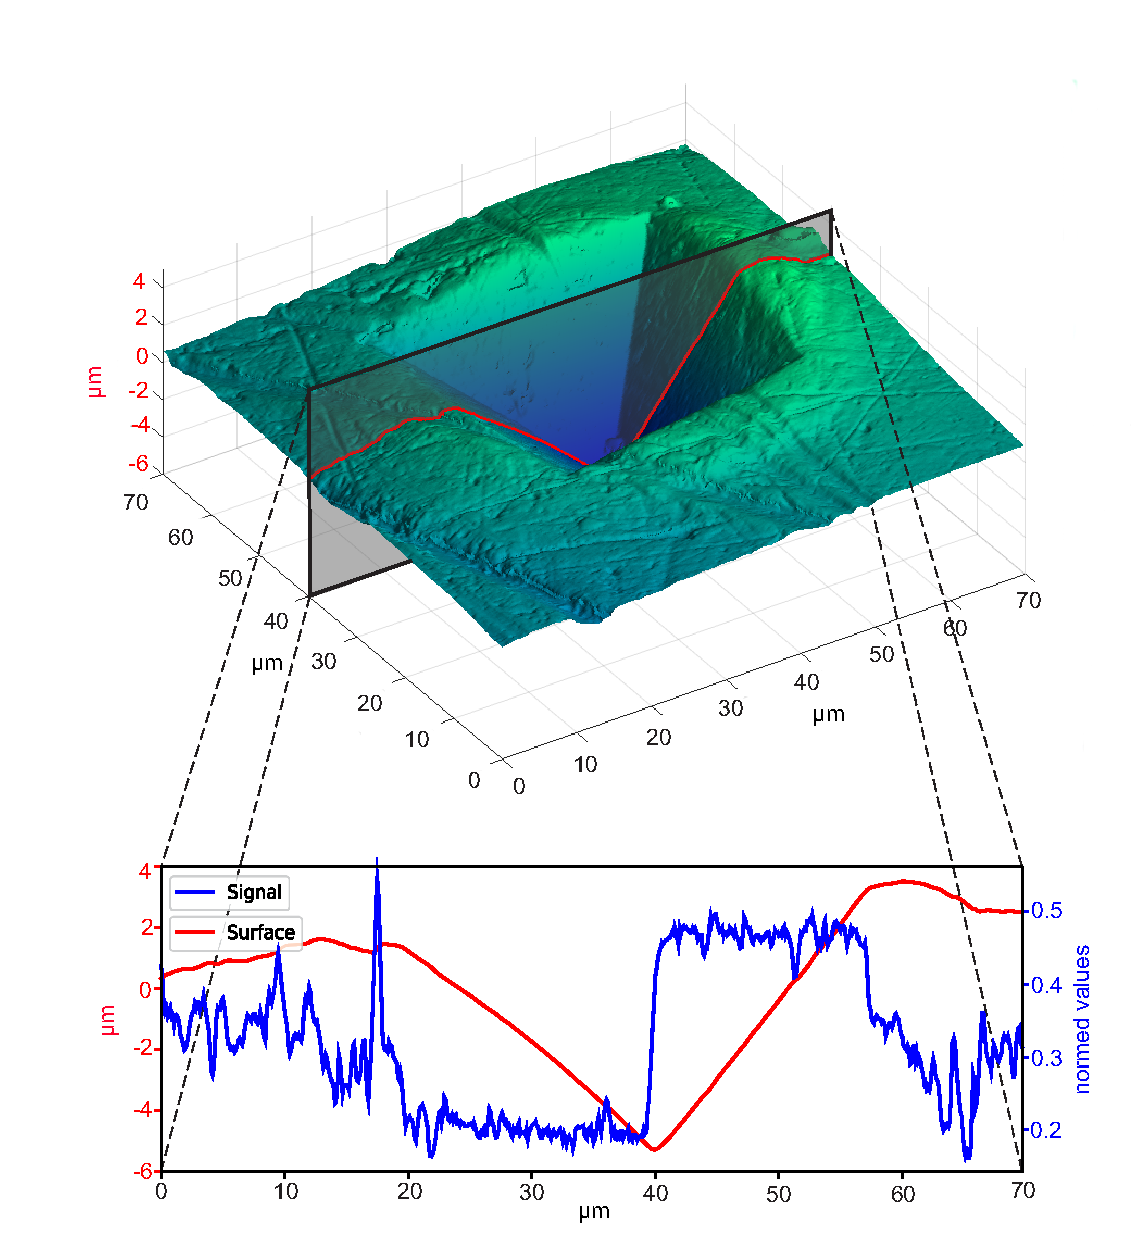
\includegraphics[width=0.45\linewidth]{indentor.eps}
        \caption{Восстановленная поверхность, входной сигнал которой изображен на
        рис.~\ref{fig:indentor-source}}
        {\label{fig:indentor}}% chktex 8
    \end{figure}

\framebreak

    \begin{figure}[ht]
        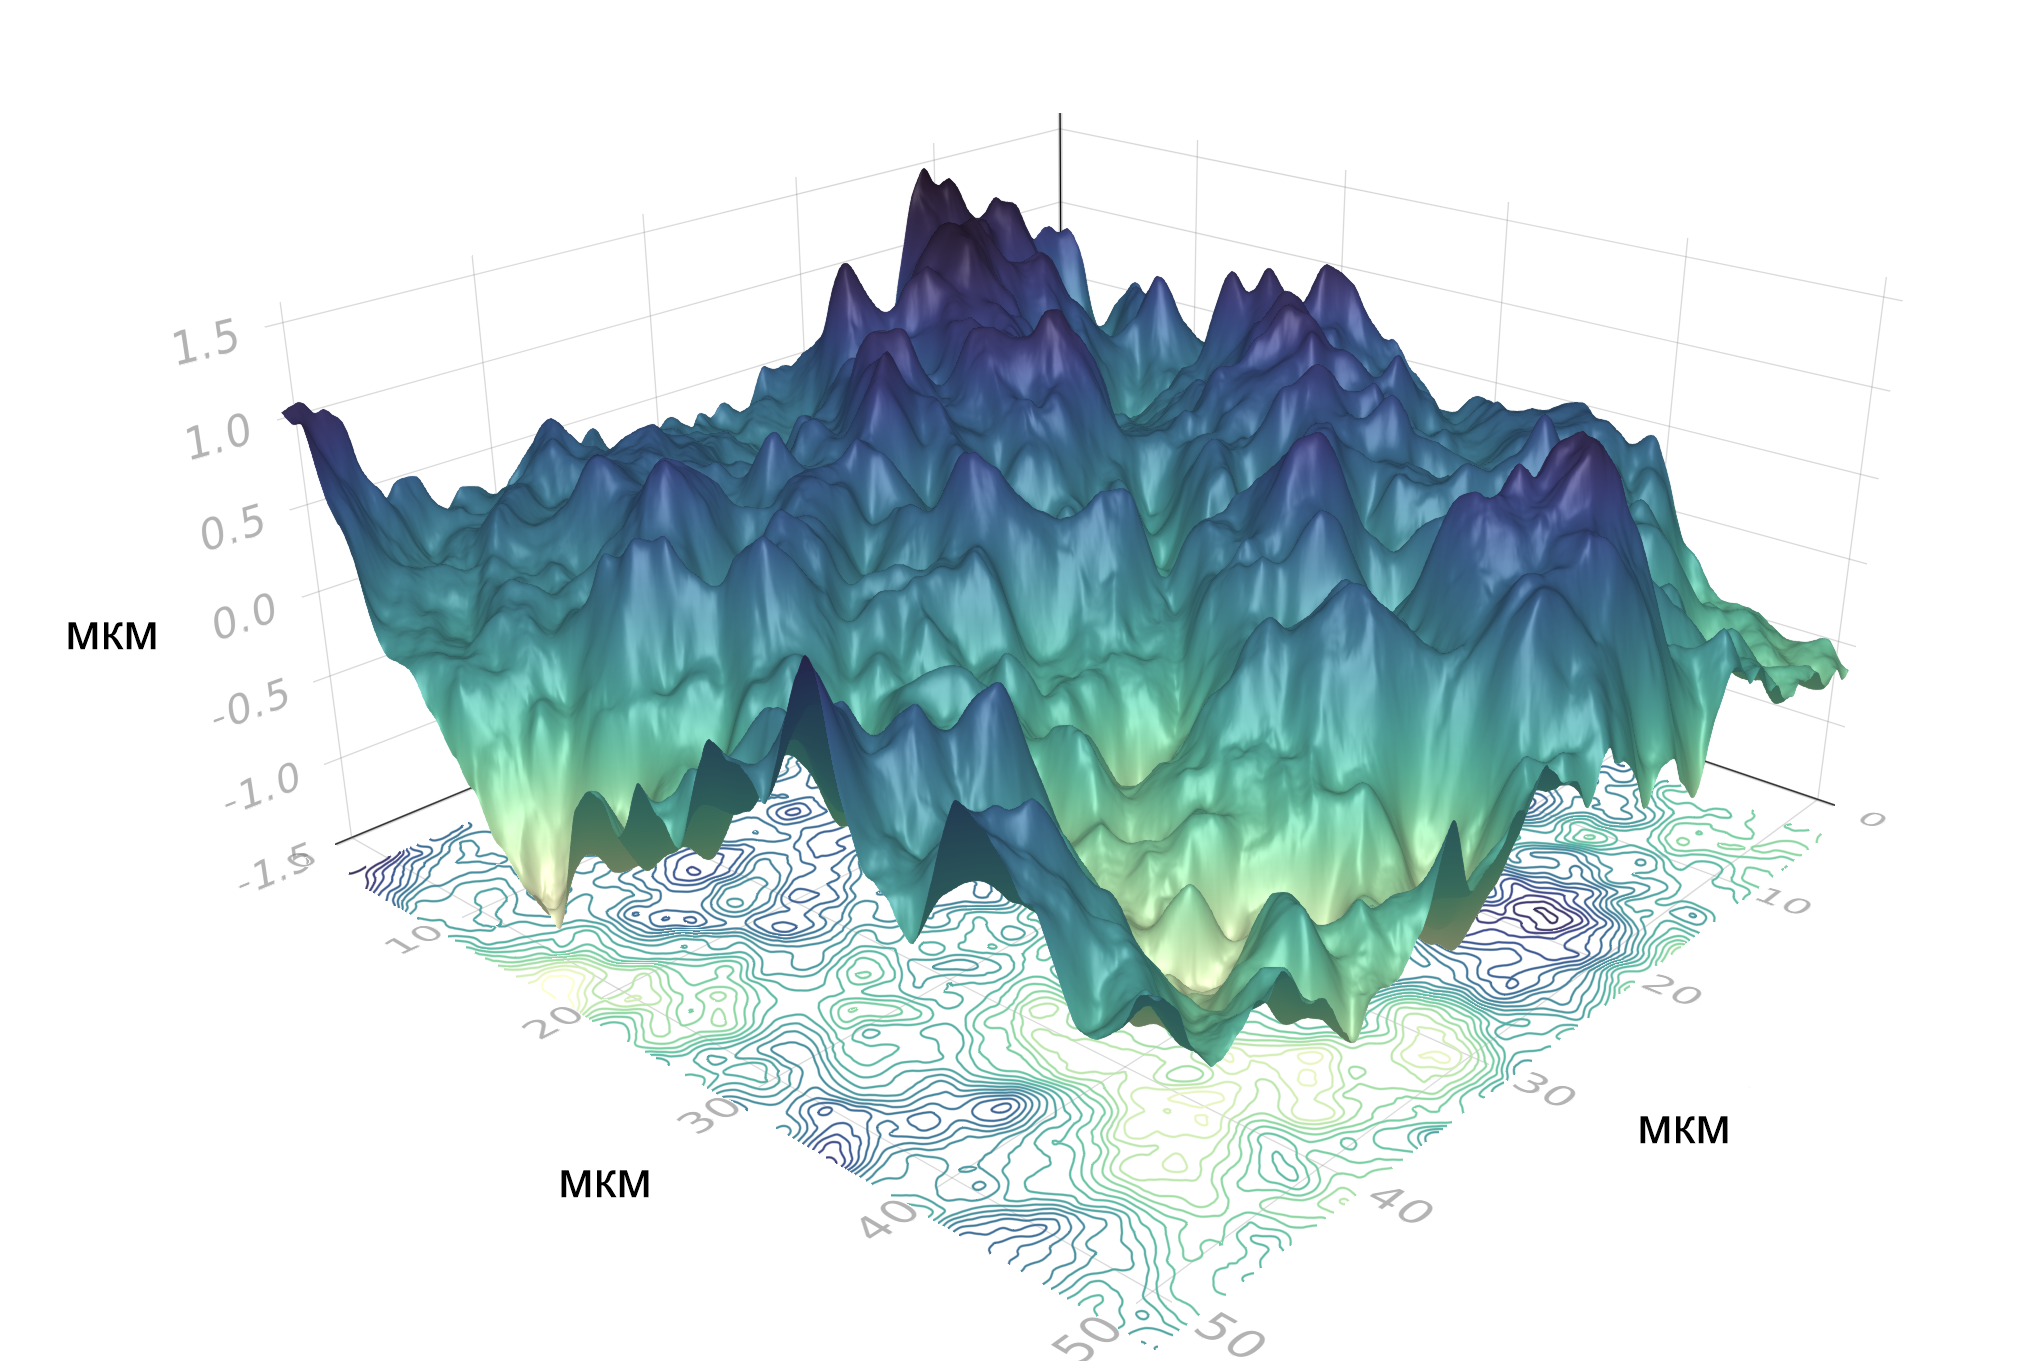
\includegraphics[width=0.55\linewidth]{PZT.png}
        \caption{Восстановленная поверхность участка пьезокерамической пластины.}
    \end{figure}


\end{frame}

\begin{frame}[c,allowframebreaks]
    \bibliography{bibliography}
\end{frame}

\begin{frame}[c]
    \frametitle{Спасибо за внимание!}
    Текст презентации доступен по ссылке
    \url{https://github.com/aborzunov/20210421}
    \begin{figure}
        
\includegraphics[width=0.5\linewidth]{repo_link.png}
    \end{figure}
    \usebeamerfont{institute} Контакты: \url{Andrey.Borzunov@gmail.com}
\end{frame}

\end{document}
